\documentclass{article}

\usepackage{standalone}
\usepackage{basicreq}
\usepackage{./teaching_doc_macros}
\usepackage{amsmath}
\usepackage{tikz}
\usetikzlibrary{arrows.meta,
                chains,
                positioning,
                shapes.geometric
                }
\title{Lecture 1: Introduction}
\author{Shashank Vatedka}


\begin{document}

%FILL IN THE RIGHT INFO.
%\lecture{**LECTURE-NUMBER**}{**UNIT**}{**LECTURER**}{**SCRIBE**}
\lecture{7}{Fano's Inequality}{Shashank Vatedka}{Aayush Goyal}

\section{Fano's inequality}

\textbf{If $M$ \& $\hat{M}$ are jointly distributed i.e. $M$,$\hat{M} \in \mathbb{M}$ and $P_{e} = P_{r}[M\neq \hat{M}]$} then,
\begin{itemize}
    \item $H(M|\hat{M}) \leq H_{2}(P_{e}) + P_e \log_{2}|\mathbb{M}|$
\end{itemize} 

\section{Proof}

Let $E = \left\{
        \begin{array}{ll}
            1 & \text{if } \hat{M} \neq M \\
            0 & \text{if } \hat{M} = M
        \end{array}
    \right.$
\\ \\
$H(E) &= H_{2}(P_e)$

If $M = \hat{M} \implies H(M|\hat{M}) = 0 $

If $M, \hat{M}$ are independent $\implies H(M|\hat{M} = H(M) $
\begin{flalign}
H(M,E | \hat{M}) &= H(M|\hat{M}) + H(E|M,\hat{M}) && \\
H(M,E | \hat{M}) &= H(E|\hat{M}) + H(M|E,\hat{M}) && \\
H(M|\hat{M}) &= H(E|\hat{M}) + H(M|E, \hat{M}) - H(E|M, \hat{M}) &&
\end{flalign}
\text{Since E is a function of $M$, $\hat{M}$}
\begin{flalign}
H(M|\hat{M}) &= H(E|\hat{M}) + H(M|E, \hat{M}) - 0 &&
\end{flalign}
\text{Conditioning reduces entropy}
\begin{flalign}
H(M|\hat{M}) &\leq H(E) + H(M|E, \hat{M}) && \\
H(M|\hat{M}) &\leq  H_{2}(P_e) + H(M|E = 0, \hat{M}) P_E(0) + H(M|E = 1, \hat{M}) P_E(1) &&\\
H(M|\hat{M}) &\leq H_{2}(P_e) + H(M|\hat{M}, E=1)P_e && \\
H(M|\hat{M}) &\leq H_{2}(P_e) + P_eH(M) && \\ 
H(M|\hat{M}) &\leq H_{2}(P_e) + P_e \log_{2}|\mathbb{M}| && 
\end{flalign}

\section{Converse of channel coding theorem}
Let $M^{k_n} \in \{0,1\}^{k_n}$ be uniformly distributed

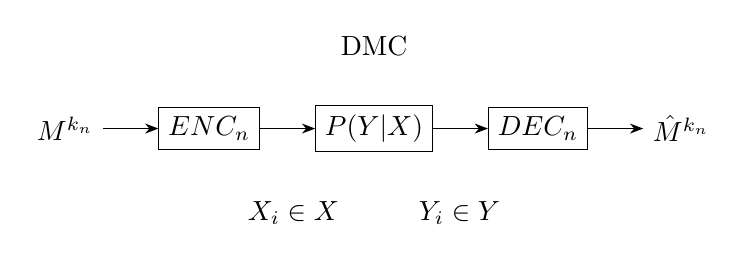
\begin{tikzpicture}[
     node distance = 5mm and 7mm,
       start chain = going right,
   alg/.style = {draw, align=center, font=\linespread{0.8}\selectfont}
                     ]
    \begin{scope}[every node/.append style={on chain, join=by -Stealth}]
    \node (n1)  {$M^{k_n}$};
    \node (n2) [alg]  {$ENC_n$};
    \node (n3) [alg]  {$P(Y|X)$};
    \node (n4) [alg] {$DEC_n$};
    \node (n5)  {$\hat{M}^{k_n}$};
    \end{scope}
    \node[above=of n3] {DMC};
    \node[below=of n3]  {$X_i\in\mathbb{X}$\hspace{.4in}$Y_i\in\mathbb{Y}$};
\end{tikzpicture}

$C = \max\limits_{P_x} I(X;Y)$

Consider any sequence $ENC_n, DEC_n$ such that
 
$\lim_{n \to \infty} inf \dfrac{k_n}{n} \geq c + \epsilon$

Then,

$\lim_{n \to \infty} inf Pr[\hat{M}^{k_n} \neq M^{k_n}]$

\end{document}



